\documentclass[border=9pt]{standalone}
\usepackage[fontset=fandol]{ctex}
\usepackage{amsmath,amssymb,tikz}
\usetikzlibrary{arrows.meta,calc,decorations.pathmorphing}
\tikzset{arr/.style={-{Stealth[length=2mm]},semithick}}
\begin{document}

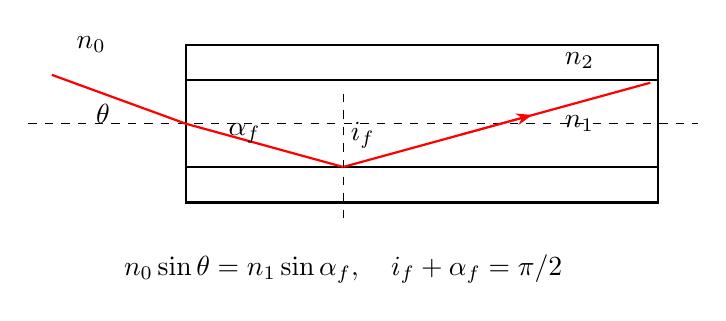
\begin{tikzpicture}
\draw[thick] (0,-1) rectangle(6,1);
\draw[thick] (0,-.55)--(6,-.55); \draw[thick] (0,.55)--(6,.55);
\draw[dashed] (-2,0)--(6.5,0);
\draw[thick,red] (-1.7,.62)--(0,0)--(2,-.55)--(5.9,.52);
\draw[arr,red] (3.5,-.138)--(4.4,.11);
\draw[dashed] (2,-1.2)--(2,.4);
\node at(-1.05,.12) {$\theta$};\node at(.75,-.12) {$\alpha_f$};
\node at(2.25,-.15) {$i_f$};
\node at(5,0) {$n_1$};\node at(5,.8) {$n_2$};\node at(-1.2,1) {$n_0$};
\node at(2,-1.85) {$n_0\sin\theta=n_1\sin\alpha_f,\quad i_f+\alpha_f=\pi/2$};
\end{tikzpicture}

\end{document}
